\chapter{Realistic Soft Shadow Mapping}
\label{chap:shadows}

\section{Two-Pass Shadow Mapping Architecture}
Hard shadows produce unrealistic, razor-sharp silhouettes and severe aliasing artifacts. To achieve visual fidelity, \textit{Matsuri Nights} incorporates an optimized two-pass \textbf{Percentage-Closer Filtering (PCF) Soft Shadow Mapping} system.

\subsection{Pass 1: Directional Light Depth Generation}
In the first render pass (\texttt{Scene::renderShadowDepth}):
\begin{enumerate}
    \item An offscreen Framebuffer Object (FBO), \texttt{depthMapFBO}, is bound with dimensions $2048 \times 2048$.
    \item A single 2D depth texture, \texttt{depthMap}, formatted as \texttt{GL\_DEPTH\_COMPONENT}, is attached. The texture wrap modes are configured to \texttt{GL\_CLAMP\_TO\_BORDER} with a border color of $[1.0, 1.0, 1.0, 1.0]^T$, ensuring fragments outside the light frustum are never falsely shadowed.
    \item \textbf{Peter-Panning Mitigation:} Hardware face culling is switched to front faces (\texttt{glCullFace(GL\_FRONT)}). Consequently, the depth buffer captures back faces, preventing self-shadowing light leakage between touching geometry.
    \item The directional light's orthographic projection matrix and view matrix are computed:
    \begin{equation}
    \mathbf{P}_{\text{ortho}} = \operatorname{ortho}(-35.0, 35.0, -25.0, 25.0, 1.0, 90.0)
    \end{equation}
    \begin{equation}
    \mathbf{V}_{\text{light}} = \operatorname{lookAt}\left( -\mathbf{D}_{\text{light}} \times 40.0\,\text{m}, \begin{bmatrix} 0 \\ 0 \\ -5 \end{bmatrix}, \begin{bmatrix} 0 \\ 1 \\ 0 \end{bmatrix} \right)
    \end{equation}
    \begin{equation}
    \mathbf{M}_{\text{lightSpace}} = \mathbf{P}_{\text{ortho}} \cdot \mathbf{V}_{\text{light}}
    \end{equation}
    \item The minimal depth shader (\texttt{shaders/shadow\_depth.vert}) transforms all non-emissive meshes into light clip space.
\end{enumerate}

\subsection{Pass 2: Shading Pass with PCF Filtering}
During the primary forward rendering pass, the generated depth map is bound to \texttt{GL\_TEXTURE1}. The fragment shader (\texttt{shaders/basic.frag: calculateShadow}) computes projected light-space coordinates:
\begin{equation}
\mathbf{p}_{\text{proj}} = \left(\frac{\mathbf{p}_{\text{lightSpace}}.xyz}{\mathbf{p}_{\text{lightSpace}}.w}\right) \cdot 0.5 + 0.5
\end{equation}
If coordinates fall outside $[0, 1]^3$, shadow occlusion is set to $0.0$.

\section{Artifact Mitigation Strategies}
\subsection{Adaptive Slope-Scale Depth Bias}
Flat bias constants fail on steep surfaces, generating either shadow acne (bias too small) or light detachment/Peter-Panning (bias too large). Equation~\ref{eq:shadow_bias} dynamically scales bias based on the angle between the surface normal $\mathbf{N}$ and incident light direction $\mathbf{L}$:
\begin{lstlisting}[language=GLSL, basicstyle=\ttfamily\scriptsize]
float bias = max(0.0035 * (1.0 - dot(normal, lightDir)), 0.0006);
\end{lstlisting}

\subsection{16-Sample PCF Convolution}
Rather than performing a binary depth comparison, the shader samples a $4\times 4$ disc kernel centered around the projected texel with texel spacing $\Delta = \frac{1.2}{2048.0}$:
\begin{lstlisting}[language=GLSL, basicstyle=\ttfamily\scriptsize]
float shadow = 0.0;
const vec2 texelSize = vec2(1.0 / 2048.0);
for(int x = -1; x <= 2; ++x) {
    for(int y = -1; y <= 2; ++y) {
        float pcfDepth = texture(shadowMap, projCoords.xy + vec2(x, y) * texelSize * 1.2).r;
        shadow += (projCoords.z - bias > pcfDepth) ? 1.0 : 0.0;
    }
}
shadow /= 16.0;
\end{lstlisting}
This filtering produces soft contact penumbrae under Machiya roof eaves, Torii crossbeams, and street stalls.

\section{Visual Verification}
Pressing the \textbf{V} key toggles shadow mapping. Figure~\ref{fig:shadows_comparison} illustrates the profound visual improvement achieved by 16-sample PCF soft shadows over unshadowed rendering.

\begin{figure}[htbp]
\centering
\begin{subfigure}[b]{0.48\textwidth}
  \centering
  \IfFileExists{figures/ss_15_shadows_disabled.png}{%
    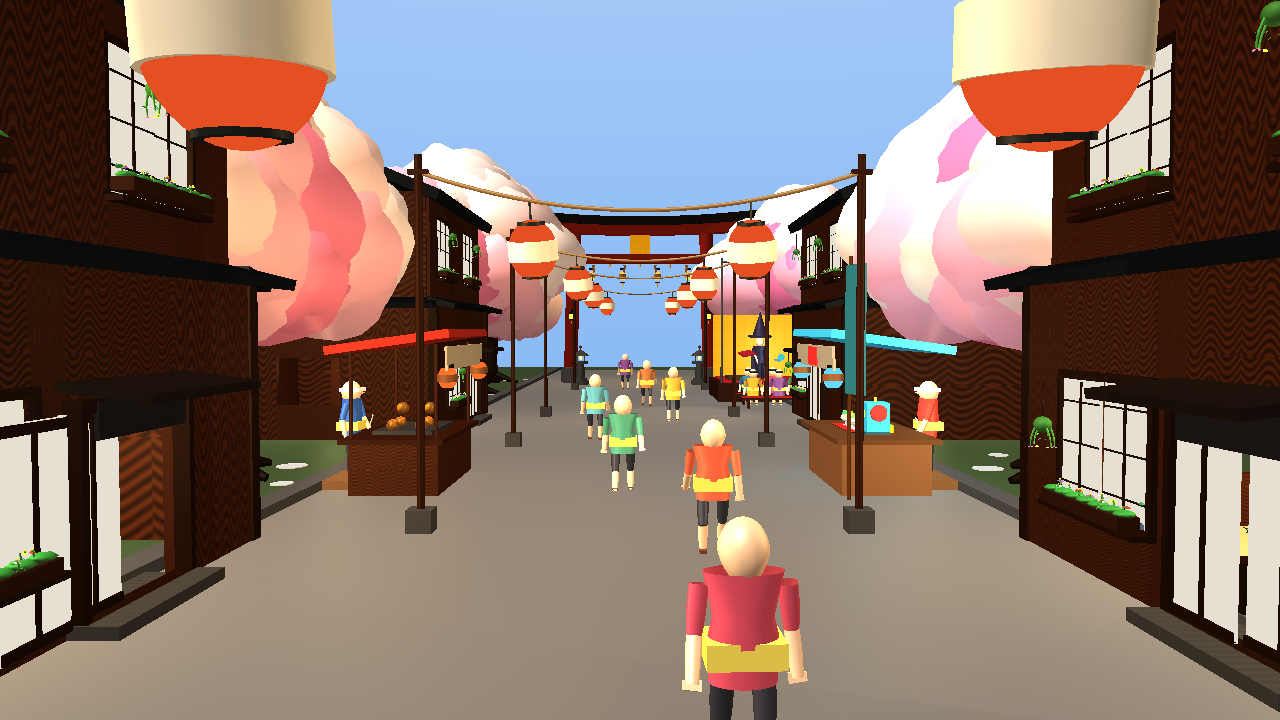
\includegraphics[width=\textwidth]{figures/ss_15_shadows_disabled.png}%
  }{\fbox{ss\_15}}
  \caption{Shadows Disabled (Flat unshadowed lighting)}
  \label{fig:shadows_off}
\end{subfigure}\hfill
\begin{subfigure}[b]{0.48\textwidth}
  \centering
  \IfFileExists{figures/ss_16_pcf_soft_shadows.png}{%
    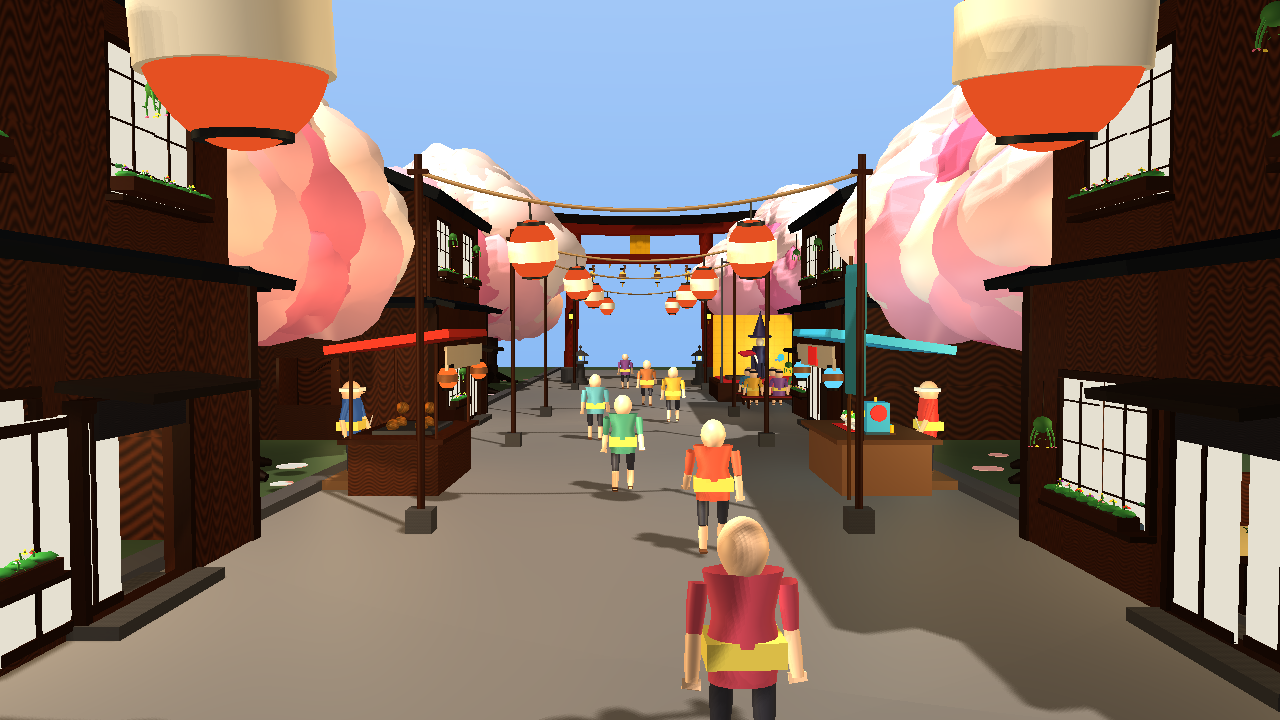
\includegraphics[width=\textwidth]{figures/ss_16_pcf_soft_shadows.png}%
  }{\fbox{ss\_16}}
  \caption{16-Sample PCF Soft Shadows Enabled}
  \label{fig:shadows_on}
\end{subfigure}
\caption{Visual impact of realistic 16-sample PCF soft shadow mapping accessible via Key V.}
\label{fig:shadows_comparison}
\end{figure}
